\documentclass{article}
\usepackage{fullpage}
\usepackage{times}
\usepackage{fancyhdr,graphicx,amsmath,amssymb}
\usepackage[ruled,vlined]{algorithm2e}
\include{pythonlisting}

\usepackage{multirow}
\usepackage{graphicx}
\usepackage{blindtext}

\usepackage{subcaption}

\usepackage{arxiv}
\usepackage{listings}
\lstset
{ %Formatting for code in appendix
    language=C,
    basicstyle=\footnotesize,
    numbers=left,
    stepnumber=1,
    showstringspaces=false,
    tabsize=1,
    breaklines=true,
    breakatwhitespace=false,
    xleftmargin=0.04\textwidth,
}
\usepackage[utf8]{inputenc} % allow utf-8 input
\usepackage[T1]{fontenc}    % use 8-bit T1 fonts
\usepackage{hyperref}       % hyperlinks
\usepackage{url}            % simple URL typesetting
\usepackage{booktabs}       % professional-quality tables
\usepackage{amsfonts}       % blackboard math symbols
\usepackage{nicefrac}       % compact symbols for 1/2, etc.
\usepackage{microtype}      % microtypography
\usepackage{lipsum}
\newcommand*\samethanks[1][\value{footnote}]{\footnotemark[#1]}
\newcommand{\tabincell}[2]{\begin{tabular}{@{}#1@{}}#2\end{tabular}}
\title{Systematic Predicate Abstraction using Deep Learning}


\author{
  Name \thanks{All contributions are considered equal.}\\
  Department of \\
   University\\
  Address \\
  \texttt{xxx@xxx} \\
  %% examples of more authors
   \And
 Name \samethanks\\
  Department of \\
   University\\
  Address \\
  \texttt{xxx@xxx} \\
     \And
 Name \samethanks\\
  Department of \\
   University\\
  Address \\
  \texttt{xxx@xxx} \\
  %% \AND
  %% Coauthor \\
  %% Affiliation \\
  %% Address \\
  %% \texttt{email} \\
  %% \And
  %% Coauthor \\
  %% Affiliation \\
  %% Address \\
  %% \texttt{email} \\
  %% \And
  %% Coauthor \\
  %% Affiliation \\
  %% Address \\
  %% \texttt{email} \\
}

\begin{document}
\maketitle

\begin{abstract}
Systematic Predicate Abstraction using Deep Learning
\end{abstract}


% keywords can be removed
\keywords{First keyword \and Second keyword \and More}


\section{Introduction}
Systematic Predicate Abstraction using Deep Learning

Summarize the pipline: 

\section{Background}
---
\subsection{Abstraction Based Model Checking}
---
\subsection{CEGAR}
---
\subsection{Abstract Interpolation}
---
\section{Problem Overview}
---

\section{Data Collection}
For a single instance of data extracting, the inputs are a list of templates $T_{0},T_{1},...,T_{n}$ and a program $P$. The output is a list of templates with 0 or 1 labels $T_{0}^{l},T_{1}^{l},...,T_{n}^{l}, l= 0$ or $1$. A concrete example for an output is $T_{0}^{1} = ("inv\_main8:VerifHintInitPred(((\_0 + -1 * \_2) >= 0))",1)$

\begin{algorithm}[H]
\SetAlgoLined
\KwResult{$T_{0}^{l},T_{1}^{l},...,T_{n}^{l}$}
 initialization:  CurrentTemplateList = $\{T_{0},T_{1},...,T_{n}\}$\;
 Solvalbility=CEGAR(CurrentTemplateList,HornClauses)\;
   \eIf{Solvalbility == True}{
    \While{CurrentTemplateList is not empty}{
        CurrentTemplateList = CurrentTemplateList $ - \{T_{k}\} (0\leqslant k \leqslant n)$\;
        Solvalbility=CEGAR(CurrentTemplateList,HornClauses)\;
        \eIf{Solvalbility == True}{
            RedunantTemplatesList=RedunantTemplatesList $\cup$ $T_{k}^{0}$;\
        }{
            CriticalTemplatesList=CriticalTemplatesList $\cup$ $T_{k}^{1}$;\
        }
    }
   }{
   No need for templates\;
  }
 \caption{Data extracting process}
\end{algorithm}

The strategy $A$ (fixed time out) to extract the training data (a list of templates with labels) is that for one program, we run Eldarica with an abstraction heuristic (e.g. use option -abstract:manual for .c files and -abstract for .smt2 files). If Eldarica can solve the program within 60 seconds. We mark this program as solvable. In Eldarica, we have an initial list of templates. We delete these templates one by one to see if the program can be solved with the remaining templates. If the program is still solvable within the timeout, then that deleted template is critical, we mark it as useful and label it as 1. By doing so iteratively, we can label the initial list of templates. This labelled list of templates will be used in the training process.

\begin{enumerate}
  \item chc-comp benchmarks: 38/1216 .smt2 files (programs) need templates to solve the program within in 60 seconds.
  \item sv-comp smt benchmarks: 7/6814 .smt2 files need templates.
  \item sv-comp c benchmarks: 31/545 .c files need templates.
\end{enumerate}

Only 76 training programs in total.

A alternative strategy $B$ (variable timeout): First, confirm the solvability (i.e. the program can be solved within 60 seconds with the abstraction heuristic).
Second, record the solving time with and without the abstraction heuristic. If Eldarica takes less solving time with abstraction heuristic, pass this solving time as timeout to Eldarica to label the templates used in the program.

\begin{enumerate}
  \item chc-comp benchmarks: 40/1216.  32 programs (204 templates)for training and 8 (47 templates) for testing. 8/8 solved by read templates. Read templates time consumption/original templates consumption =  40.25/40.86 (in seconds)
  \item sv-comp smt benchmarks: 15/5911.  12 programs (254 templates)for training and 3 (74 templates) for testing. 3/3 solved by read templates. Read templates time consumption/original templates consumption =  28.07/27.28 (in seconds)
  \item sv-comp c benchmarks: 41/555.  32 programs (4635 templates)for training and 9 (350 templates) for testing. 8/9 solved by read templates. Read templates time consumption/original templates consumption = 34.04/53.46  (in seconds)
\end{enumerate}

96 training programs. 76 programs for training, 20 programs for testing.
18/20 solved by read templates. Read templates time consumption/original templates consumption =  140.67/126.84 (in seconds)

Strategy $C$: keep using Strategy $B$'s on larger benchmarks, and use these three benchmarks only for testing.

\begin{center}
\begin{tabular}{lp{1cm}p{1cm}p{1.5cm}p{1.5cm}p{1.5cm}p{1.5cm}p{1.5cm}}
\hline
Benchmarks & File type & Total file & Solved with abstract (abstract:manual) & Unsolved with abstract (abstract:manual)& Training program (templates) & Testing program (templates) &Solved by read templates\\
\hline
chc-comp & .smt2 & 1216 & -&-&-&-&-\\
sv-comp smt & .sm2 & 5911 & -&-&-&-&-\\
sv-comp C & .c & 555 & - &-&-&-&-\\
In total  & .c,.smt2 & - & -&-&-&-&-\\
\hline
\end{tabular}
\end{center}

\section{Training Model}


\begin{figure}[h]
\centering
  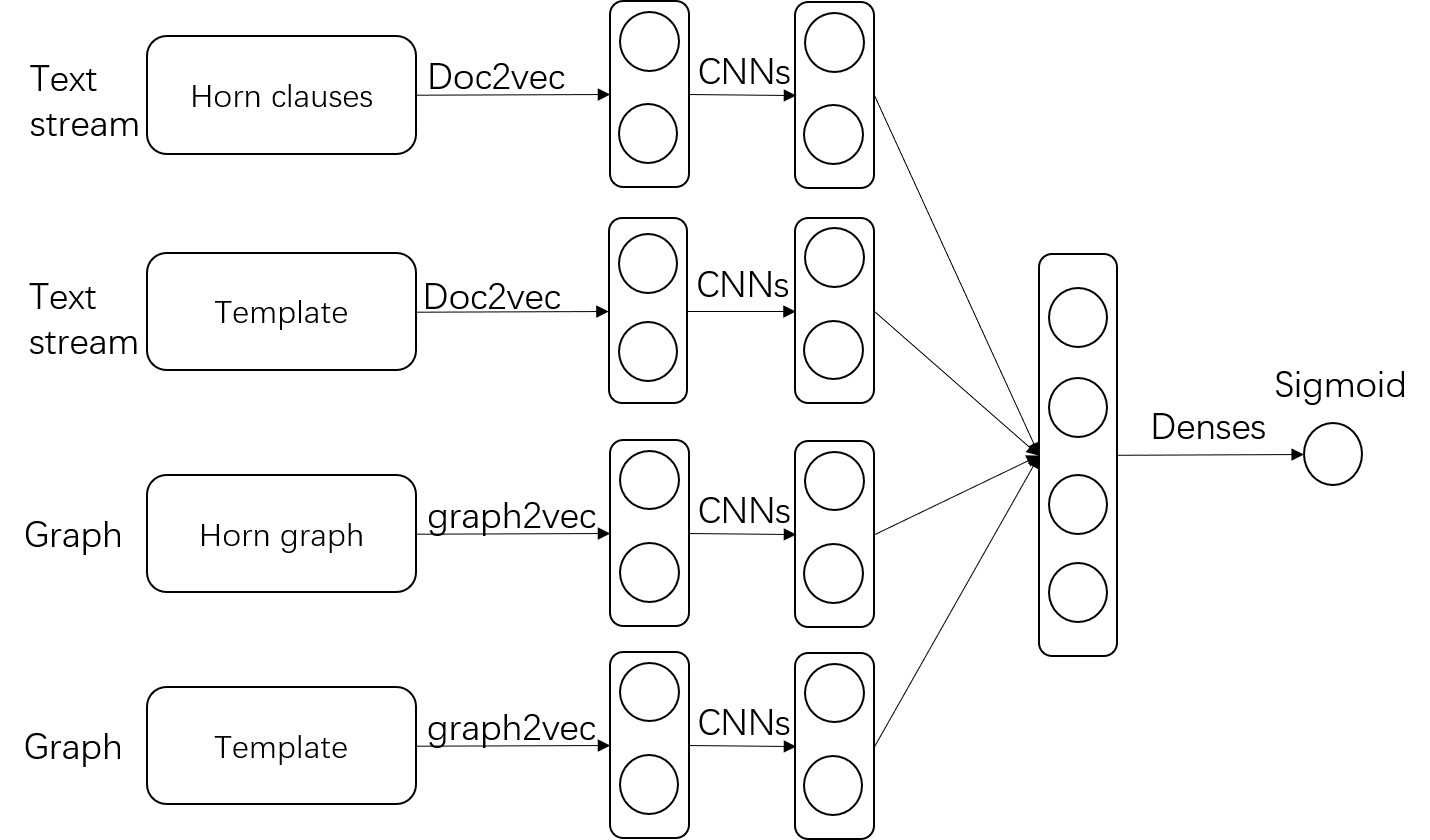
\includegraphics[width=10cm]{graph/NNstructure}\\
  \caption{Neural network structure}\label{NNstructure}
\end{figure}
\subsection{Program Embedding}

\subsubsection{Text Level}
Doc2Vec \cite{DBLP:journals/corr/LeM14} embed different length of sentences to fixed vector.
Program text streams are embedded into 100 dimensions. Template text streams are embedded to 20 dimensions.
\subsubsection{Graph Level}
Graph2Vec\cite{DBLP:journals/corr/NarayananCVCLJ17}.
WL relabeling process \cite{WL_relabeling_process} to generate random subgraphs (can be seen as sentences). Then use Doc2Vec embed subgraphs to fixed vector.
Program graphs (horn graphs) are embedded into 100 dimensions. Templates are embedded to 20 dimensions.
\subsubsection{Graph Representation}

Each template contain location, category, and predicate information. One example template is "inv\_main8:VerifHintInitPred(((\_0 + -1 * \_2) >= 0))" in which "inv\_main8" is its control location,"VerifHintInitPred" is its category (The meaning of the categories can be found in appendix), and "(((\_0 + -1 * \_2) >= 0))" is the predicate. \_0 and \_2 are canonical encoding of variable names in source code. For example, \_0 is x and \_2 is y.  We can combine the three components into one graph. The root node contains the location information ("inv\_main8") as its node attribute. The only child of the root contains the category information ("VerifHintInitPred"). The predicate ("(((\_0 + -1 * \_2) >= 0))") can be represent as a binary tree. We connect the binary tree's root to the category node to connect all parts together. One example is shown in Figure \ref{templateGraph}. We use graphviz to manipulate the graph. The corresponding graphviz text representation of the template is shown in \ref{templateGraphviz}
\begin{figure}[h]
\centering
\begin{subfigure}{0.3\textwidth}
\begin{lstlisting}
digraph dag {
0 [label="inv_main8/4"];
1 [label="VerifHintInitPred"];
2 [label=">="];
3 [label="0"];
4 [label="+"];
5 [label="_0"];
6 [label="*"];
7 [label="-1"];
8 [label="_2"];
0->1
1->2
2->4
2->3
4->6
4->5
6->8
6->7
\end{lstlisting}\subcaption{Template graph example in graphviz format}\label{templateGraphviz}
\end{subfigure}   ~~~~~~~~~~~~
\begin{subfigure}{0.3\textwidth}
  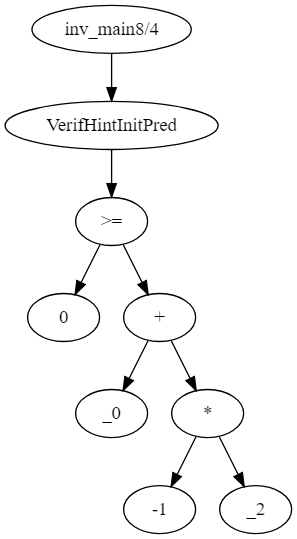
\includegraphics[width=3.4cm]{graph/template_graph}\\
  \subcaption{Template graph example}\label{templateGraph}
  \end{subfigure}
  \caption{Graph representation for an example template "inv\_main8:VerifHintInitPred(((\_0 + -1 * \_2) >= 0))"}
\end{figure}



\begin{figure}[h]
\begin{subfigure}[b]{0.4\textwidth}
\begin{lstlisting}
extern int n;
void main(){
    int x,y;
    assume(x==n,y==n);
    while(x!=0){
        x--;
        y--;
    }
    assert(y==0);
}
\end{lstlisting}\subcaption{C program for horn graph example}\label{horn_graph_while-C}
\end{subfigure}
\begin{subfigure}[b]{0.4\textwidth}
  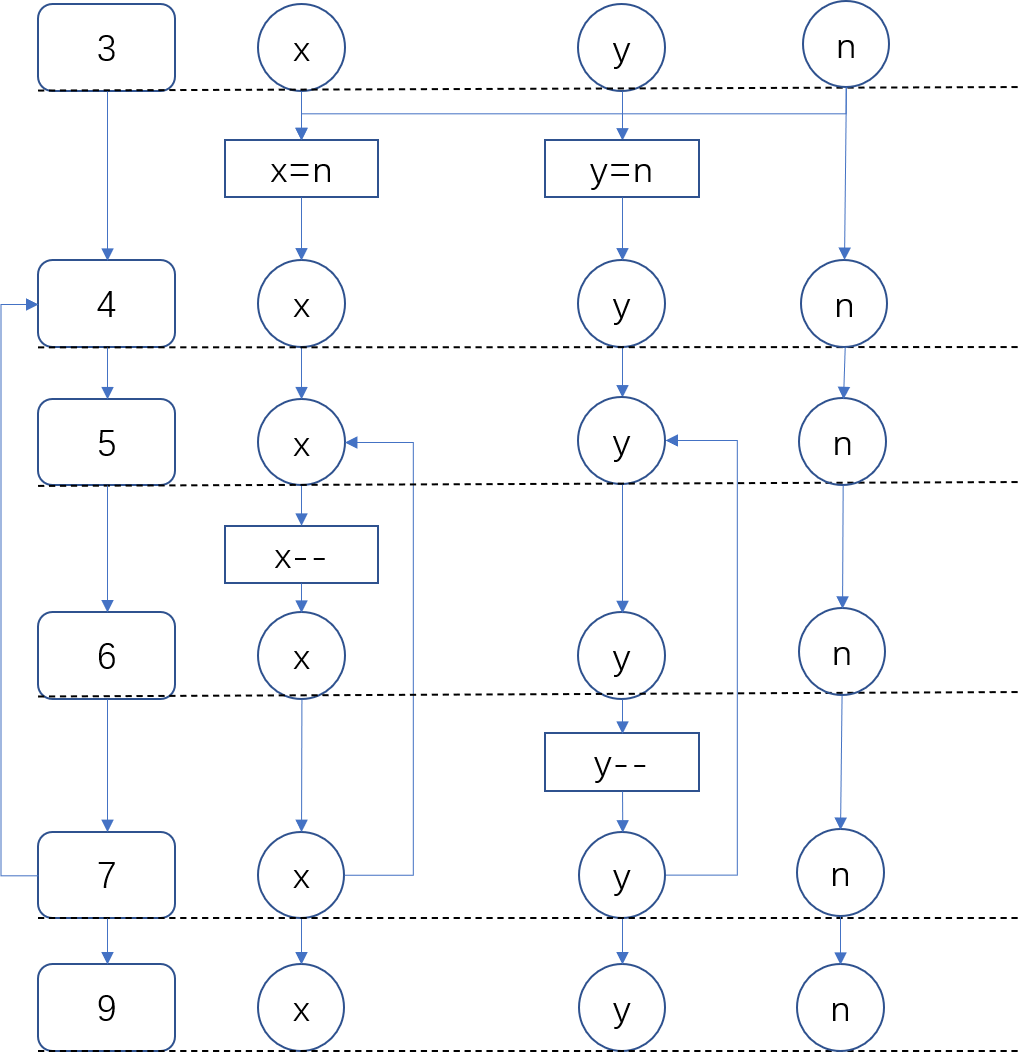
\includegraphics[width=8cm]{graph/horn_graph_while}\\
  \subcaption{Horn graph example}\label{horn_graph_while}
  \end{subfigure}
  \caption{}
\end{figure}


\section{Experiments}
The predicted result is a score for a template. We add two rank modes to decide which templates will be used for solving a particular program. For example, we have 10 templates, their scores ranged from 0 to 1. The first rank mode can specify a threshold for the scores. If the threshold is 0.4, all templates that have scores larger than 0.4 will be used to solve the program, and the left templates are discarded. The second rank mode can specify a hierarchical number (N) which decides to use top N ranked templates by score. If we specify the hierarchical number (N) be 5, then the top 5 ranked templates by score will be used to solve the program, and the left 5 templates will be discarded.

Solvability:
\begin{center}
\begin{tabular}{lp{1cm}p{1cm}p{1cm}p{1cm}p{1cm}p{1cm}p{1cm} }
\hline
Benchmarks & File type & Total file & with template graph & with horn graph & with control flow graph &with control flow and template graphs & with horn and template graphs\\
\hline
chc-comp & .smt2 & 1216 & -&-\\
sv-comp smt & .sm2 & 5911 & -&-\\
sv-comp C & .c & 555 & -&-\\
\hline
\end{tabular}
\end{center}

Time consumption:
\begin{center}
\begin{tabular}{lp{1cm}p{1cm}p{1cm}p{1cm}p{1cm}p{1cm}p{1cm} }
\hline
Benchmarks & File type & Total file & with template graph & with horn graph & with control flow graph &with control flow and template graphs & with horn and template graphs\\
\hline
chc-comp & .smt2 & 1216 & -&-\\
sv-comp smt & .sm2 & 5911 & -&-\\
sv-comp C & .c & 555 & -&-\\
\hline
\end{tabular}
\end{center}

\section{Related work}
Program synthesis:

Logical reasoning: NEO, BLAZE, CEGIS.

Machine learning methods:
Program synthesis from examples:
Encode inputs to fixed vector, then decode this vector to target language.

Program induction:
Directly give output. The learned program is induced latently within the weights and activations of a neural network.

Guide formal method's search process by Training a statistical model to rank some options existed in search space and try them first.


\section{Discussion and Future work}
%
%
%\section{Headings: first level}
%\label{sec:headings}
%
%\lipsum[4] See Section \ref{sec:headings}.
%
%\subsection{Headings: second level}
%\lipsum[5]
%\begin{equation}
%\xi _{ij}(t)=P(x_{t}=i,x_{t+1}=j|y,v,w;\theta)= {\frac {\alpha _{i}(t)a^{w_t}_{ij}\beta _{j}(t+1)b^{v_{t+1}}_{j}(y_{t+1})}{\sum _{i=1}^{N} \sum _{j=1}^{N} \alpha _{i}(t)a^{w_t}_{ij}\beta _{j}(t+1)b^{v_{t+1}}_{j}(y_{t+1})}}
%\end{equation}
%
%\subsubsection{Headings: third level}
%\lipsum[6]
%
%\paragraph{Paragraph}
%\lipsum[7]
%
%\section{Examples of citations, figures, tables, references}
%\label{sec:others}
%\lipsum[8] \cite{kour2014real,kour2014fast} and see \cite{hadash2018estimate}.
%
%The documentation for \verb+natbib+ may be found at
%\begin{center}
%  \url{http://mirrors.ctan.org/macros/latex/contrib/natbib/natnotes.pdf}
%\end{center}
%Of note is the command \verb+\citet+, which produces citations
%appropriate for use in inline text.  For example,
%\begin{verbatim}
%   \citet{hasselmo} investigated\dots
%\end{verbatim}
%produces
%\begin{quote}
%  Hasselmo, et al.\ (1995) investigated\dots
%\end{quote}
%
%\begin{center}
%  \url{https://www.ctan.org/pkg/booktabs}
%\end{center}
%
%
%\subsection{Figures}
%\lipsum[10]
%See Figure \ref{fig:fig1}. Here is how you add footnotes. \footnote{Sample of the first footnote.}
%\lipsum[11]
%
%\begin{figure}
%  \centering
%  \fbox{\rule[-.5cm]{4cm}{4cm} \rule[-.5cm]{4cm}{0cm}}
%  \caption{Sample figure caption.}
%  \label{fig:fig1}
%\end{figure}
%
%\subsection{Tables}
%\lipsum[12]
%See awesome Table~\ref{tab:table}.
%
%\begin{table}
% \caption{Sample table title}
%  \centering
%  \begin{tabular}{lll}
%    \toprule
%    \multicolumn{2}{c}{Part}                   \\
%    \cmidrule(r){1-2}
%    Name     & Description     & Size ($\mu$m) \\
%    \midrule
%    Dendrite & Input terminal  & $\sim$100     \\
%    Axon     & Output terminal & $\sim$10      \\
%    Soma     & Cell body       & up to $10^6$  \\
%    \bottomrule
%  \end{tabular}
%  \label{tab:table}
%\end{table}
%
%\subsection{Lists}
%\begin{itemize}
%\item Lorem ipsum dolor sit amet
%\item consectetur adipiscing elit.
%\item Aliquam dignissim blandit est, in dictum tortor gravida eget. In ac rutrum magna.
%\end{itemize}


\bibliographystyle{unsrt}
%\bibliography{references}  %%% Remove comment to use the external .bib file (using bibtex).
%%% and comment out the ``thebibliography'' section.

\bibliography{references}
%%% Comment out this section when you \bibliography{references} is enabled.
%\begin{thebibliography}{1}
%
%\bibitem{kour2014real}
%George Kour and Raid Saabne.
%\newblock Real-time segmentation of on-line handwritten arabic script.
%\newblock In {\em Frontiers in Handwriting Recognition (ICFHR), 2014 14th
%  International Conference on}, pages 417--422. IEEE, 2014.
%
%\bibitem{kour2014fast}
%George Kour and Raid Saabne.
%\newblock Fast classification of handwritten on-line arabic characters.
%\newblock In {\em Soft Computing and Pattern Recognition (SoCPaR), 2014 6th
%  International Conference of}, pages 312--318. IEEE, 2014.
%
%\bibitem{hadash2018estimate}
%Guy Hadash, Einat Kermany, Boaz Carmeli, Ofer Lavi, George Kour, and Alon
%  Jacovi.
%\newblock Estimate and replace: A novel approach to integrating deep neural
%  networks with existing applications.
%\newblock {\em arXiv preprint arXiv:1804.09028}, 2018.
%
%\end{thebibliography}


\end{document}
